\subsubsection{Parsing}
\label{sec:view_parse}

\paragraph{}
Once files have been uploaded, the user needs to parse them into ROME datafiles. As discussed in section \ref{sec:controller_parser} multiple parsers may be installed. The parse page is listed under the session tab of the default ROME navigation bar. The page initial comprises a form with a simple select element, allowing the user to choose form the available parsers. The form submits via AJAX to an action in the Parser controller (section \ref{sec:controller_parser}) which returns a list of the files in the user's upload directory recognised by the selected parser. This list is in the form of a series of checkboxes and is inserted into an empty div on the parser page so the user can choose the files they wish to use, as illustrated in figure \ref{figure:parser_view}.


\begin{figure}[h]
\centering
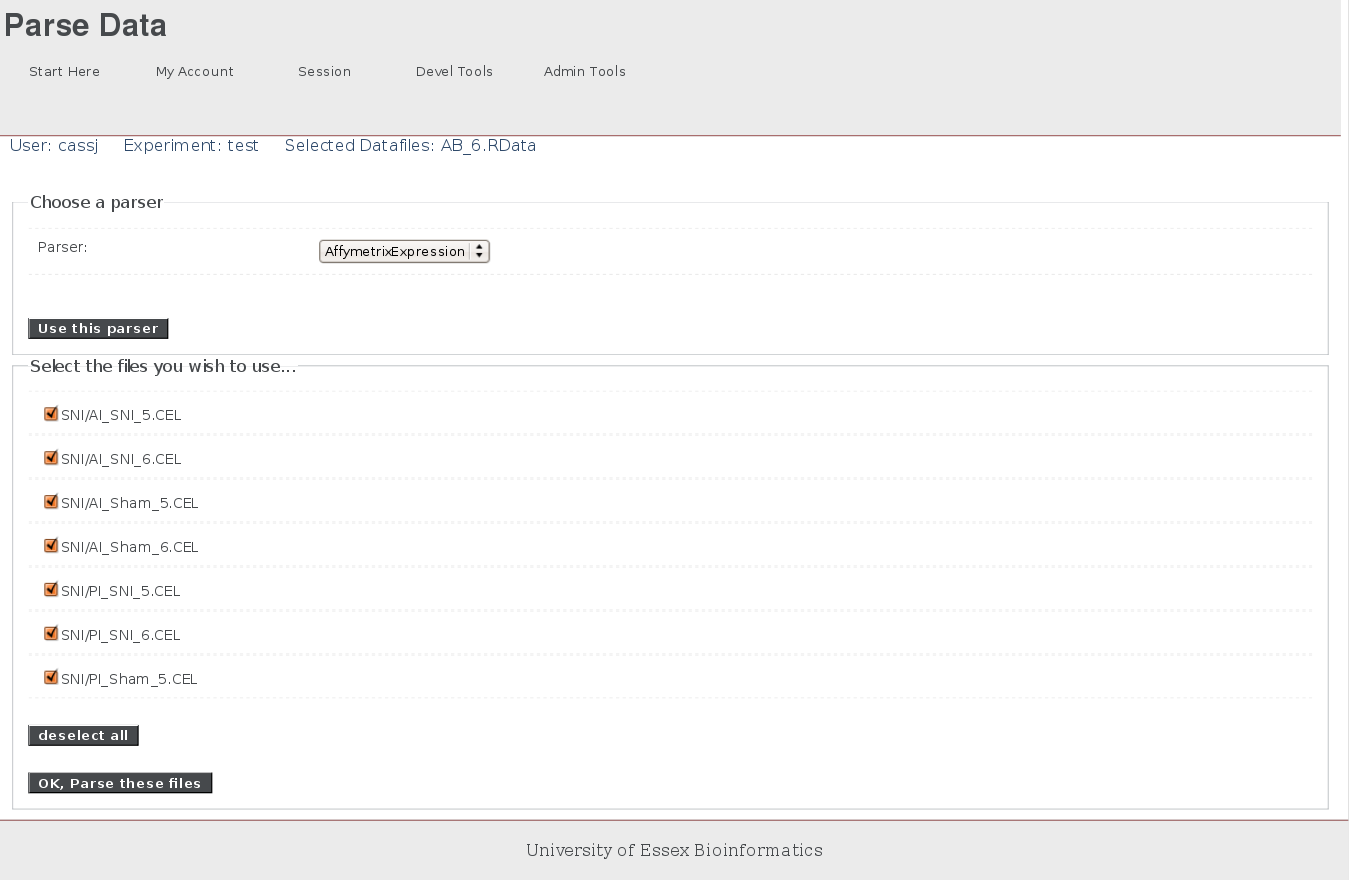
\includegraphics[scale=0.45, angle=90]{../rome/docs/images/screenshots/parse}
\caption{The Parser Page}\label{fig:parser_view}
\end{figure}

\clearpage
